%
%
\subsection{Versuchsaufbau}
In der Photozelle (Abbildung \ref{fig:Photozelle} ) findet der zu untersuchende Photoeffekt statt.
Die Photozelle wird dazu mit Licht einer bestimmten Wellenlänge und einer bestimmten
Frequenz belichtet. In einem Abstand von wenigen Millimetern zur Kathode befindet sich die Anode die in der Photozelle als kreisförmiger Drahtring darstellt.

\begin{figure}[h]
	\centering
		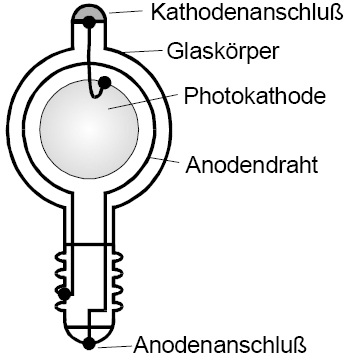
\includegraphics[width=0.30\textwidth]{Photozelle.jpg}
		\caption{Die Photozelle}
	\label{fig:Photozelle}
\end{figure}

Anhand der sogenannten Gegenfeldmethode wird die Energie der Elektronen bestimmt. Dazu
legt man eine Spannung $U_B$(Abbildung \ref{fig:PrinzipDesPhotoeffekts} ) , zwischen Anode und Kathode an, die
die emittierten Elektronen abbremst. Aus diesem Grund erreichen die Anode nur Elektronen, die die mindest Energie $E_{kin} < e_0 \cdot U$ erreichen.
Für den fall, dass

\begin{align}
\frac{1}{2} m_0 v_2 = e_0  U_G
\end{align}

gilt, verschwindet der Strom I.
Mit der Austrittsarbeit gild für die schnellsten Elektronen nun
\begin{align}
h  \nu = e_0  U_G + A_k.
\end{align}

Mit diesen Formeln lässt sich die Grenzspannung $U_G$ in abhängigkeit von der Frequenz $\nu$ ermitteln.
Das von der Lampe emittierte Licht wird durch eine Kondensorlinse gebündelt bevor es durch die Spaltblende fällt.
Hinter dem Spalt befindet sich die Abbildungslinse, welche das Licht weiter gebündelt auf das Geradsichtprisma
lenkt. Erst jetzt ist eine Untersuchung des Photoeffekts möglich, da das Prisma
die verschiedenen Spektrallinien räumlich trennt und somit ist es möglich nur Licht einer
bestimmten Frequenz auf die Kathode zu richten.(siehe Abbildung \ref{fig:Versuchsaufbau} )

\begin{figure}[h]
	\centering
		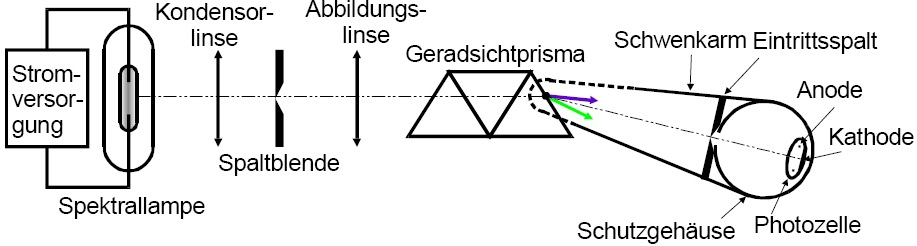
\includegraphics[width=1.00\textwidth]{Versuchsaufbau.jpg}
		\caption{Versuchsaufbau}
	\label{fig:Versuchsaufbau}
\end{figure}

\subsection{Justierung der Apperatur}
Da die zu messenden Ströme in der Größenordnung pA liegen, sind die Zuleitungen zum Picoamperemeter und
das Gehäuse der Photozelle sorgfältig gegen Störfelder abgeschirmt. Dies ist möglich durch nutzung von Koaxialkabeln,
deren Mantel auf Erdpotential liegen.Für brauchbare Messergebnisse muss man möglichst viel des von der Lampe emittierten
Lichts auf die Photokathode konzentrieren. Da die Intensität des gesammelten Lichtes stark von der Anordnung der optischen
Elemente des Versuchsaufbaus abhängt, wird im folgenden auf die Justierung der Apparatur eingegangen.
Die optischen Bauelemente müssen so angeordnet sein, dass die Kondensorlinse ein möglichst scharfes Bild in die Spaltblende einwirft,
dieses sollte die gleiche Breite wie der Spalt besitzen (ca 1- 2 mm). Zur Berechnung der Abstände können die Linsenformeln verwenden.
\begin{align}
\frac{1}{f}=\frac{1}{g}+\frac{1}{b}
\end{align}
\begin{align}
\frac{G}{B}=\frac{g}{b}
\end{align}
(f = Brennweite der Linse, g = Gegenstandsweite, b= Bildweite, G = Gegenstandsgröße, B = Bildgröße)

Entsprechendes gilt für die Abbildung der Spaltblende auf die Eintrittsöffnung der Photozelle mittels der Abbildungslinse.

\subsection{Messvorgang}
Es werden für die Messung der beiden violetten Farbtöne, sowie für Grün und Blaugrün
wird der Strom des eingestrahlte Lichts in abhängigkeit von der Gegenspannung gemessen.
Wobei die Gegenspannung im bereich von -1 Volt bis 1 Volt in 0,2 Volt schritten erhöht wird und
zwischen 1 Volt und 19 Volt in 4 Volt schritten. Dabei wird jeweils der Photostrom gemessen.

Beim Gelben Licht wird, wie bei den anderen Farben im bereich von -1 bis 19 Volt gemessen.
Zusätzlich wir aber auch im Bereich von -19 Volt bis -1 Volt in 4 Volt schritten gemessen.